In this section, we will give some details abotu how our paper view changed during implementation. 

The main issue we met is the amount of papers in the each year is quite large, which is about 150 papers per year. As a result, there is no way to arrange the entire paper view, 14 years and 100 papers per year, to one view with proper font size. The initial version of our implemention is shown as Figure~\ref{fig:pv_initial_version}.

\begin{figure}[h]			
	\centering
	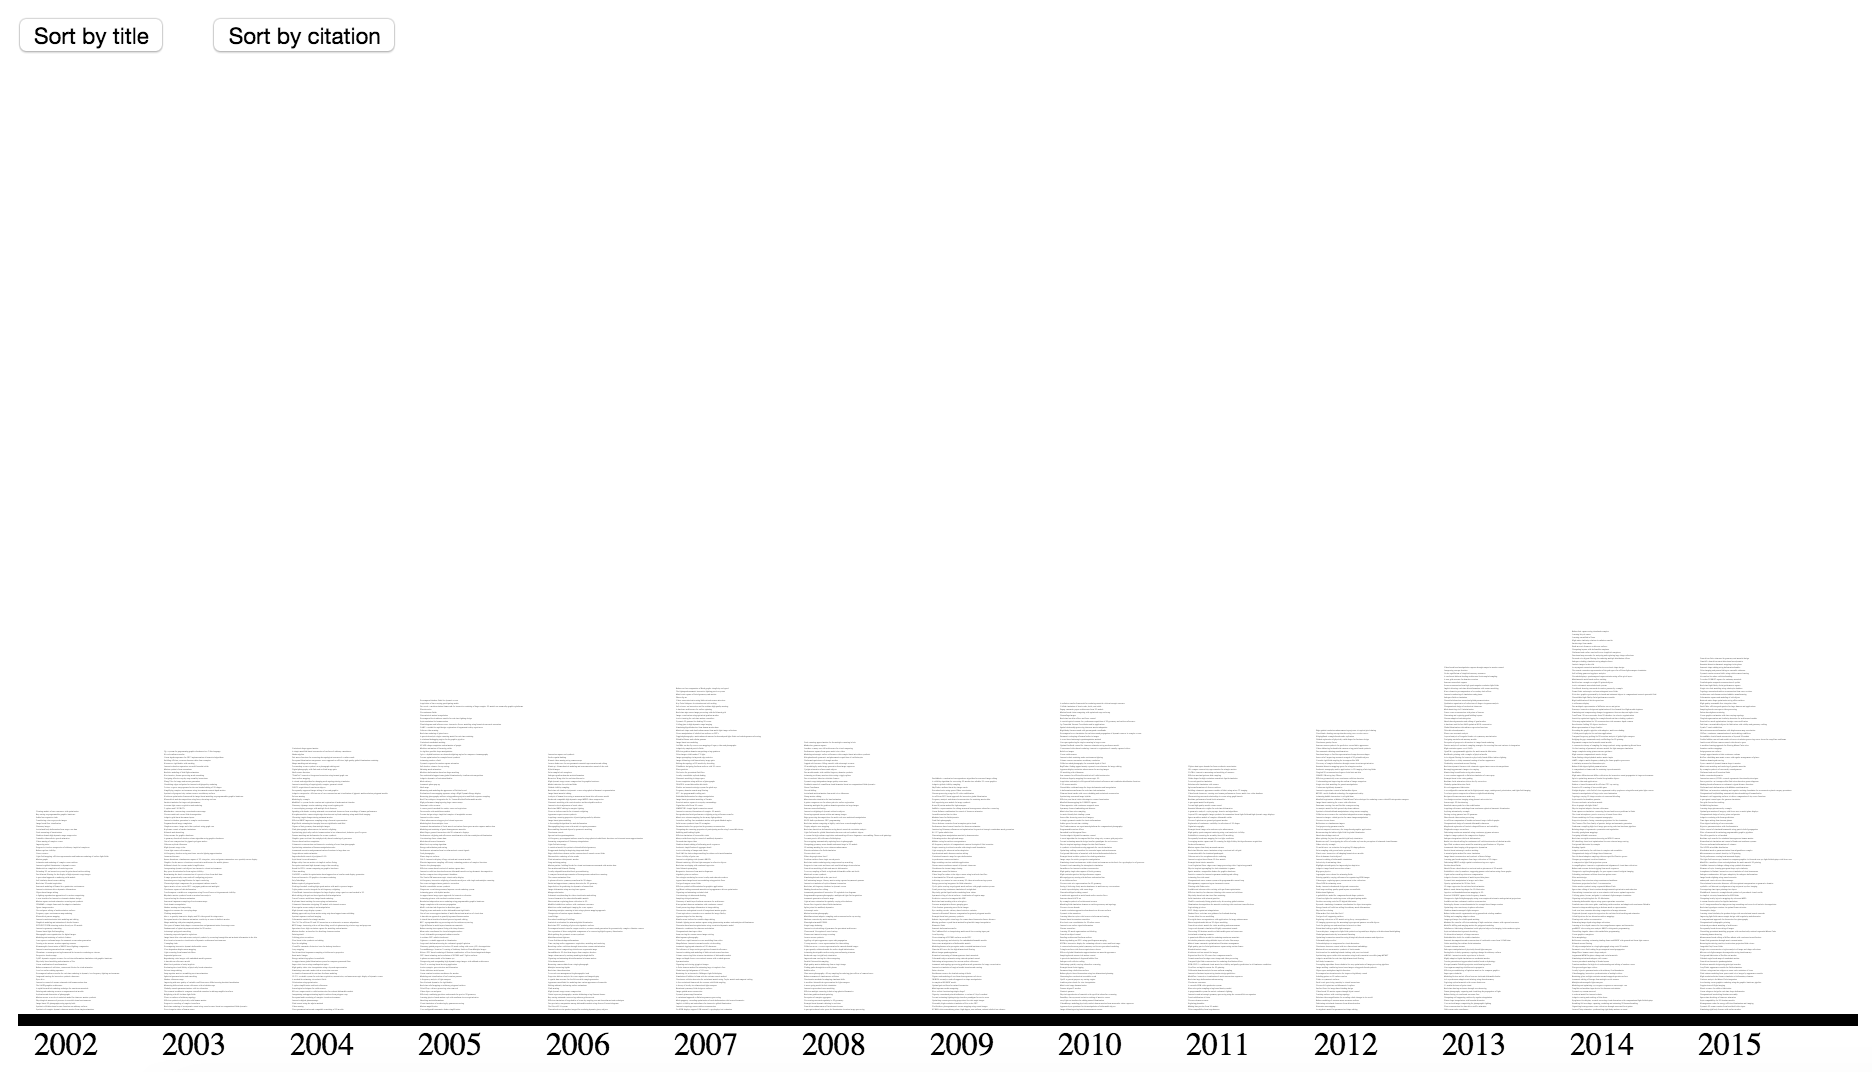
\includegraphics[width=0.7\textwidth]{paper_view_initial_version}
	\caption{The initial version of our paper view implementation}
	\label{fig:pv_initial_version}
\end{figure} 

There are two options to solve this issue. The first one is using zoom in and zoom out to let users explore paper views. We attempt to avoid that method because users may lose the entire view on their mind due to the change blindness. Hence, we added fisheye distortion to enable users to only zoom in texts in a small region as shown in Figure~\ref{fig:pv_fisheye}. However, the fisheye plugin we used is not suitable for zooming in texts. Also, because of the high density of texts, even if we rearrange texts to make it look better, it is still very messy for users to view.

\begin{figure}[ht]			
	\centering
	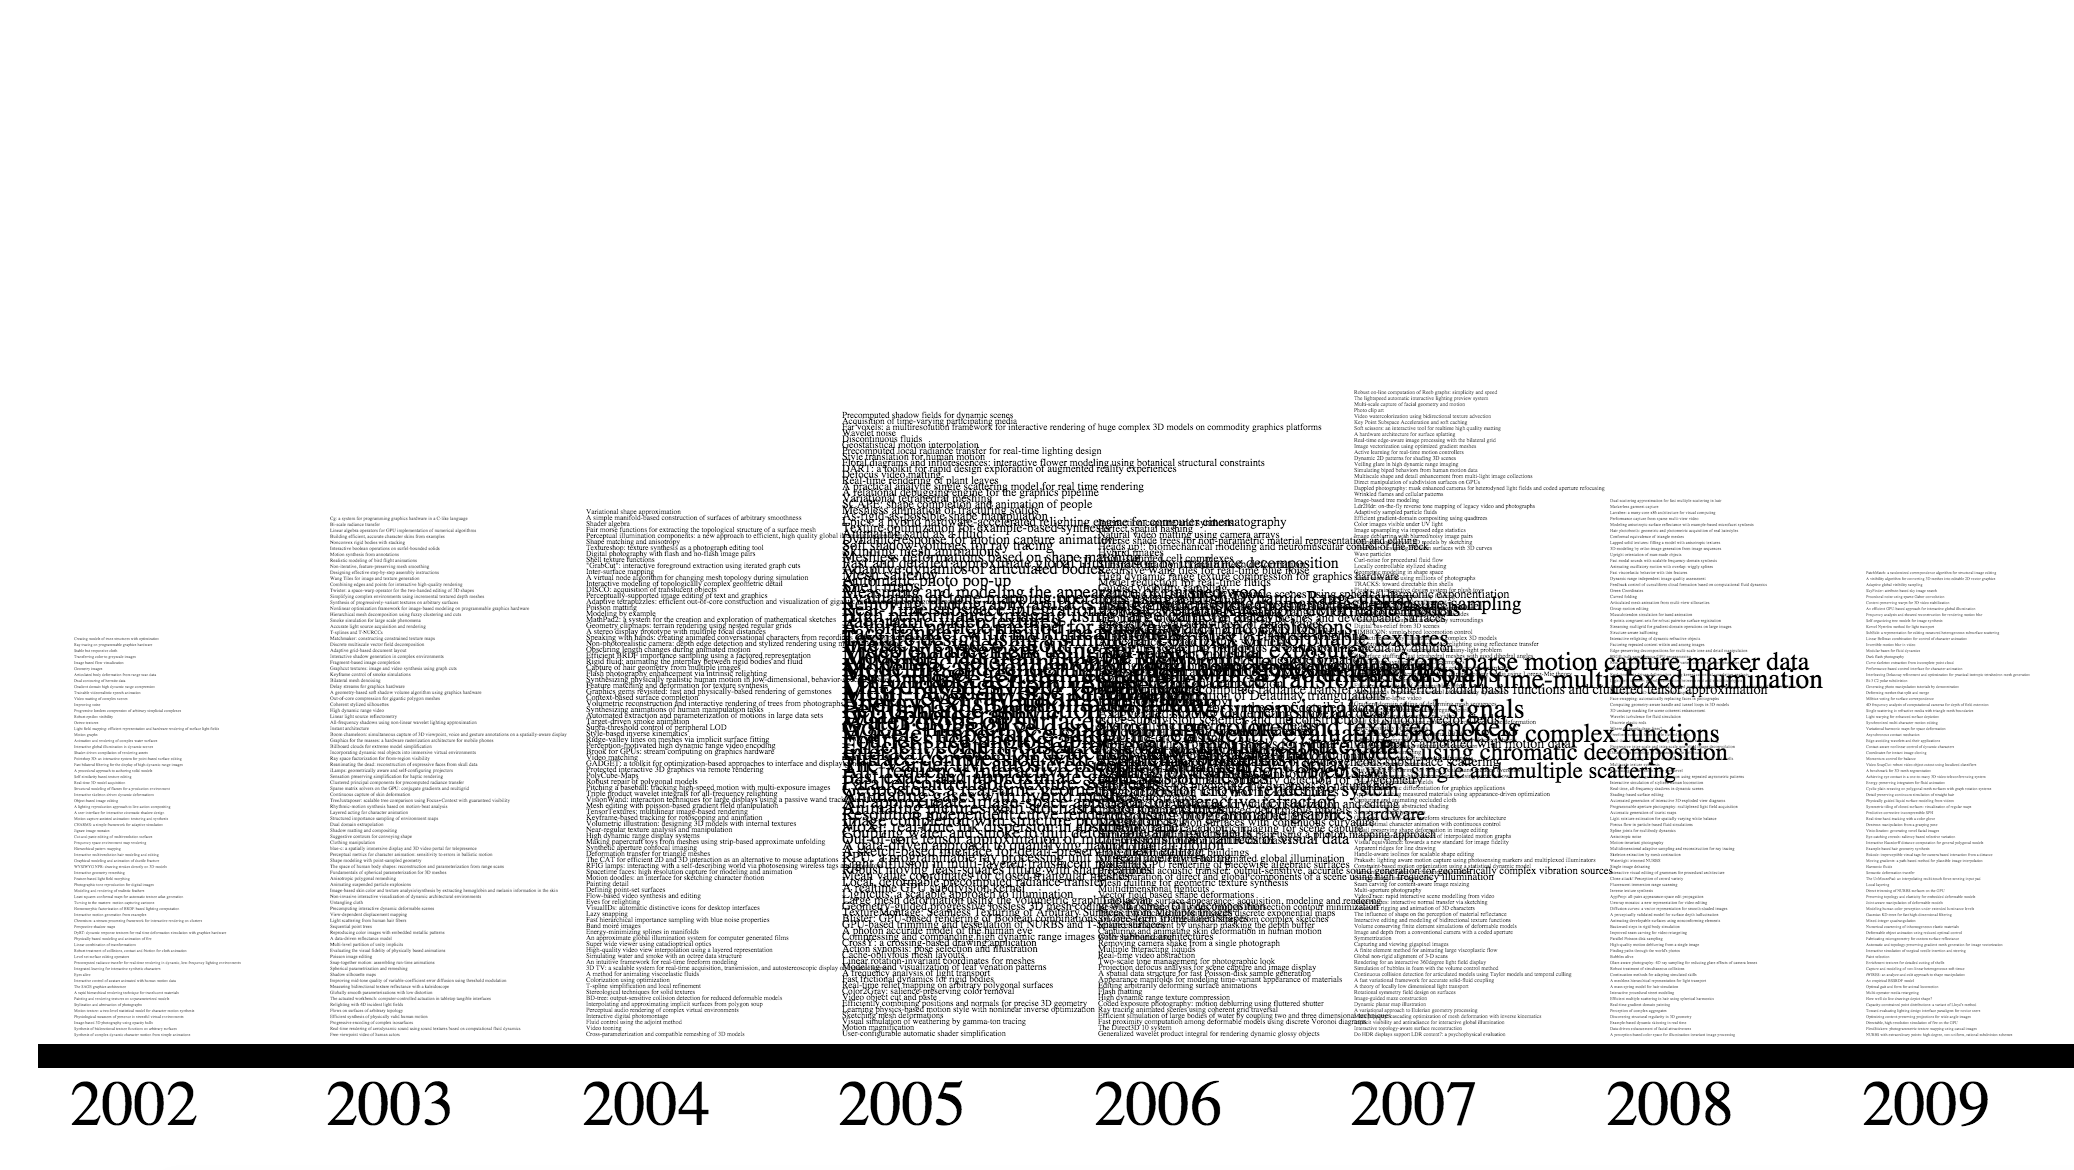
\includegraphics[width=0.7\textwidth]{paper_view_fisheye}
	\caption{Paper view with fish eye}
	\label{fig:pv_fisheye}
\end{figure} 

After that, we decided to add a side bar for the selected year papers as shown in Fgire~\ref{fig:pv_side_bar}. When users select one year, the side bar will show all papers in that year and allow users to scroll. We believe this should be the best solution for our issue without zoom in and out. Users can get details as well as overall view at the same time at least.

\begin{figure}[h]			
	\centering
	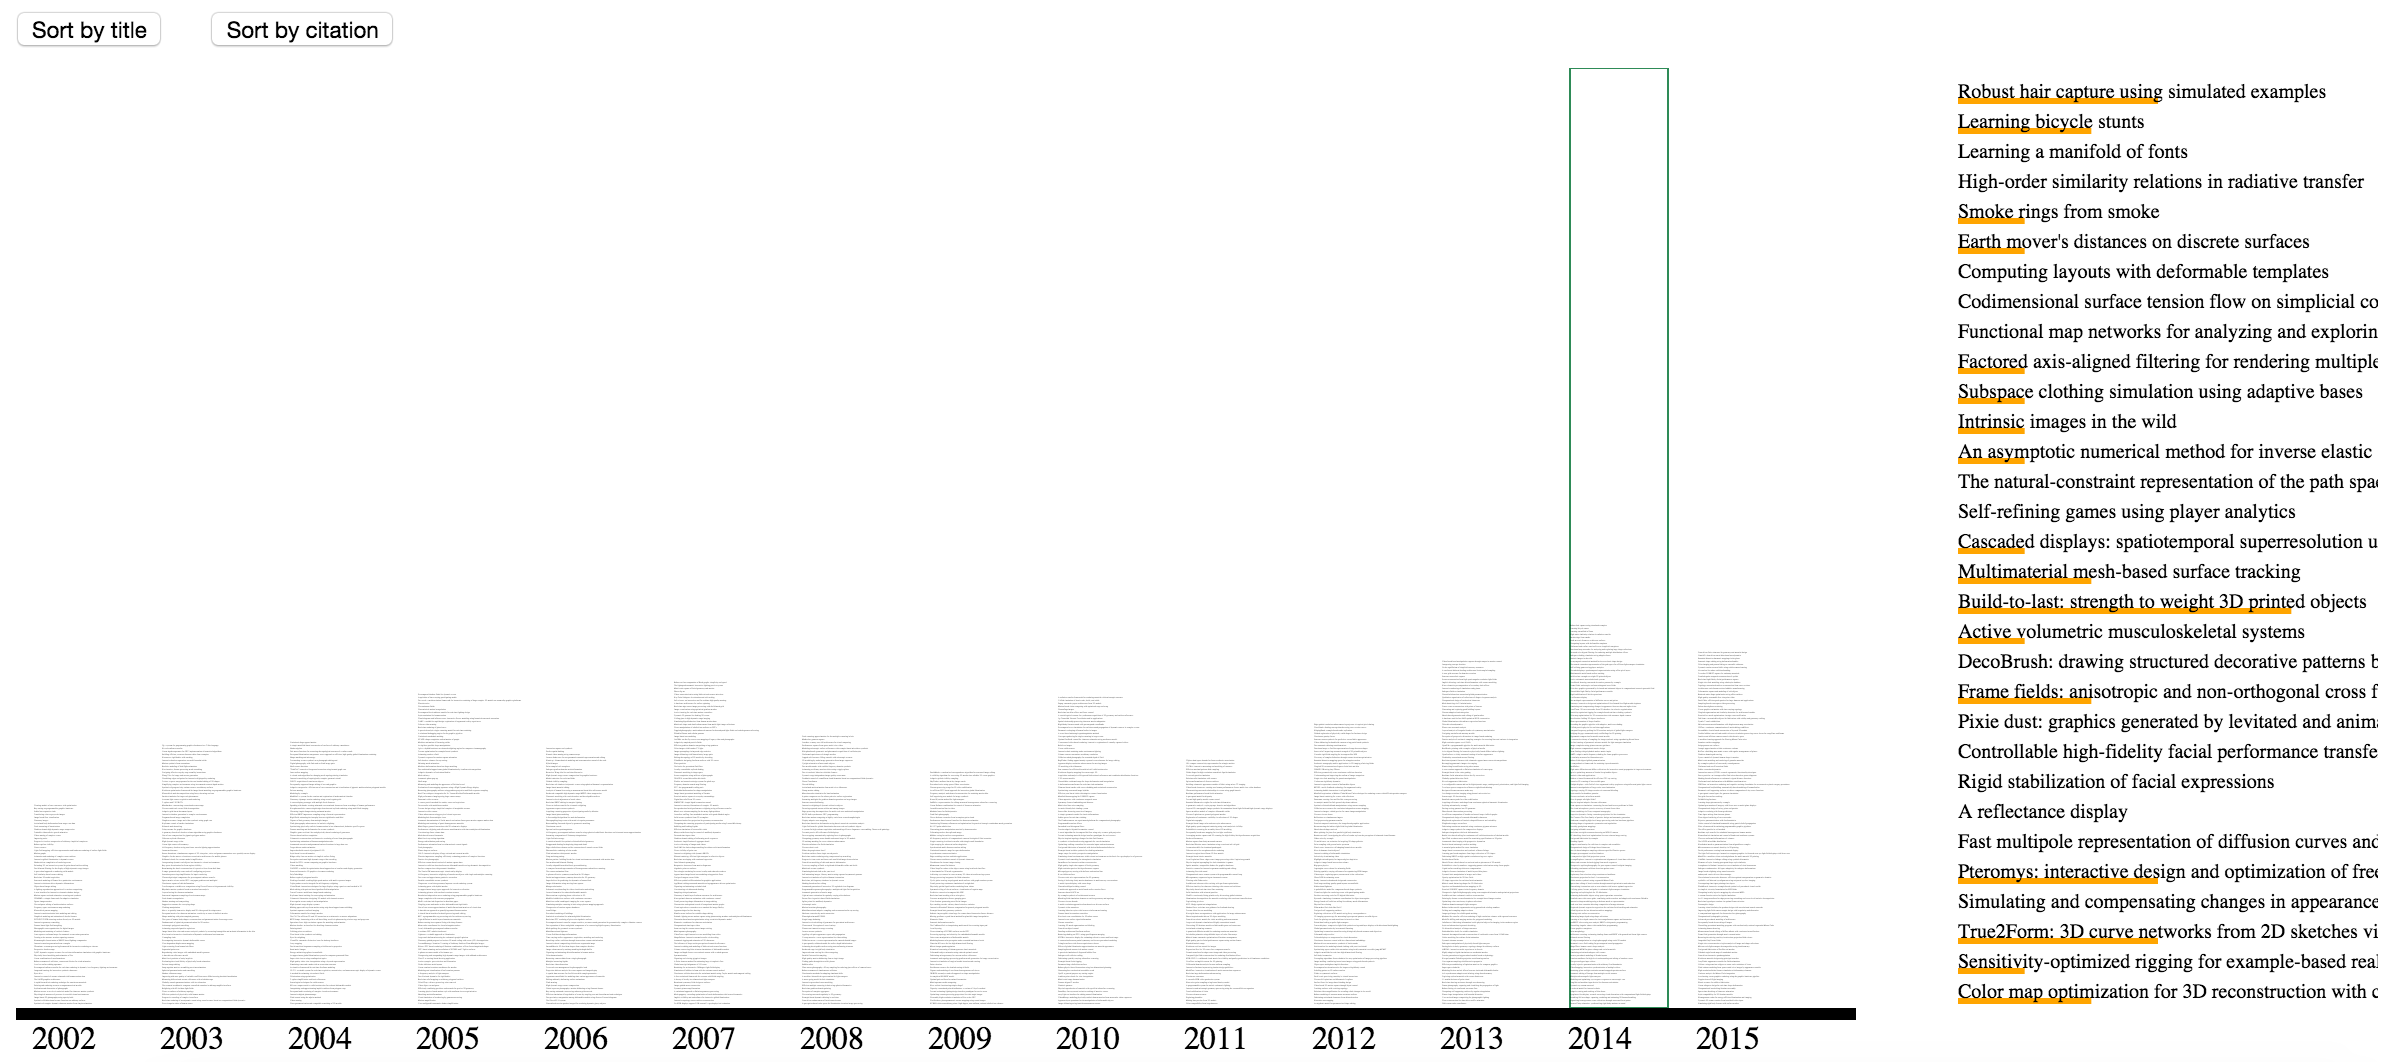
\includegraphics[width=0.7\textwidth]{paper_view_with_side_bar}
	\caption{Paper view with side bar}
	\label{fig:pv_side_bar}
\end{figure} 

However, we meet another question, which is how represent reference and citation relationship between papers in the paper view. As we mentioned before, it is too small to read and we cannot keep our original design as shown in Figure~\ref{fig:overview}. Fortunately, at the worst case, the total amount of reference and citation by one paper is 52. We determined to enlarge the font size of those papers and arrange them by stair shape as shown in Figure~\ref{fig:pv_reference_citation}. We use red and blue to highlight references and cited by papers for now.

\begin{figure}[ht]			
	\centering
	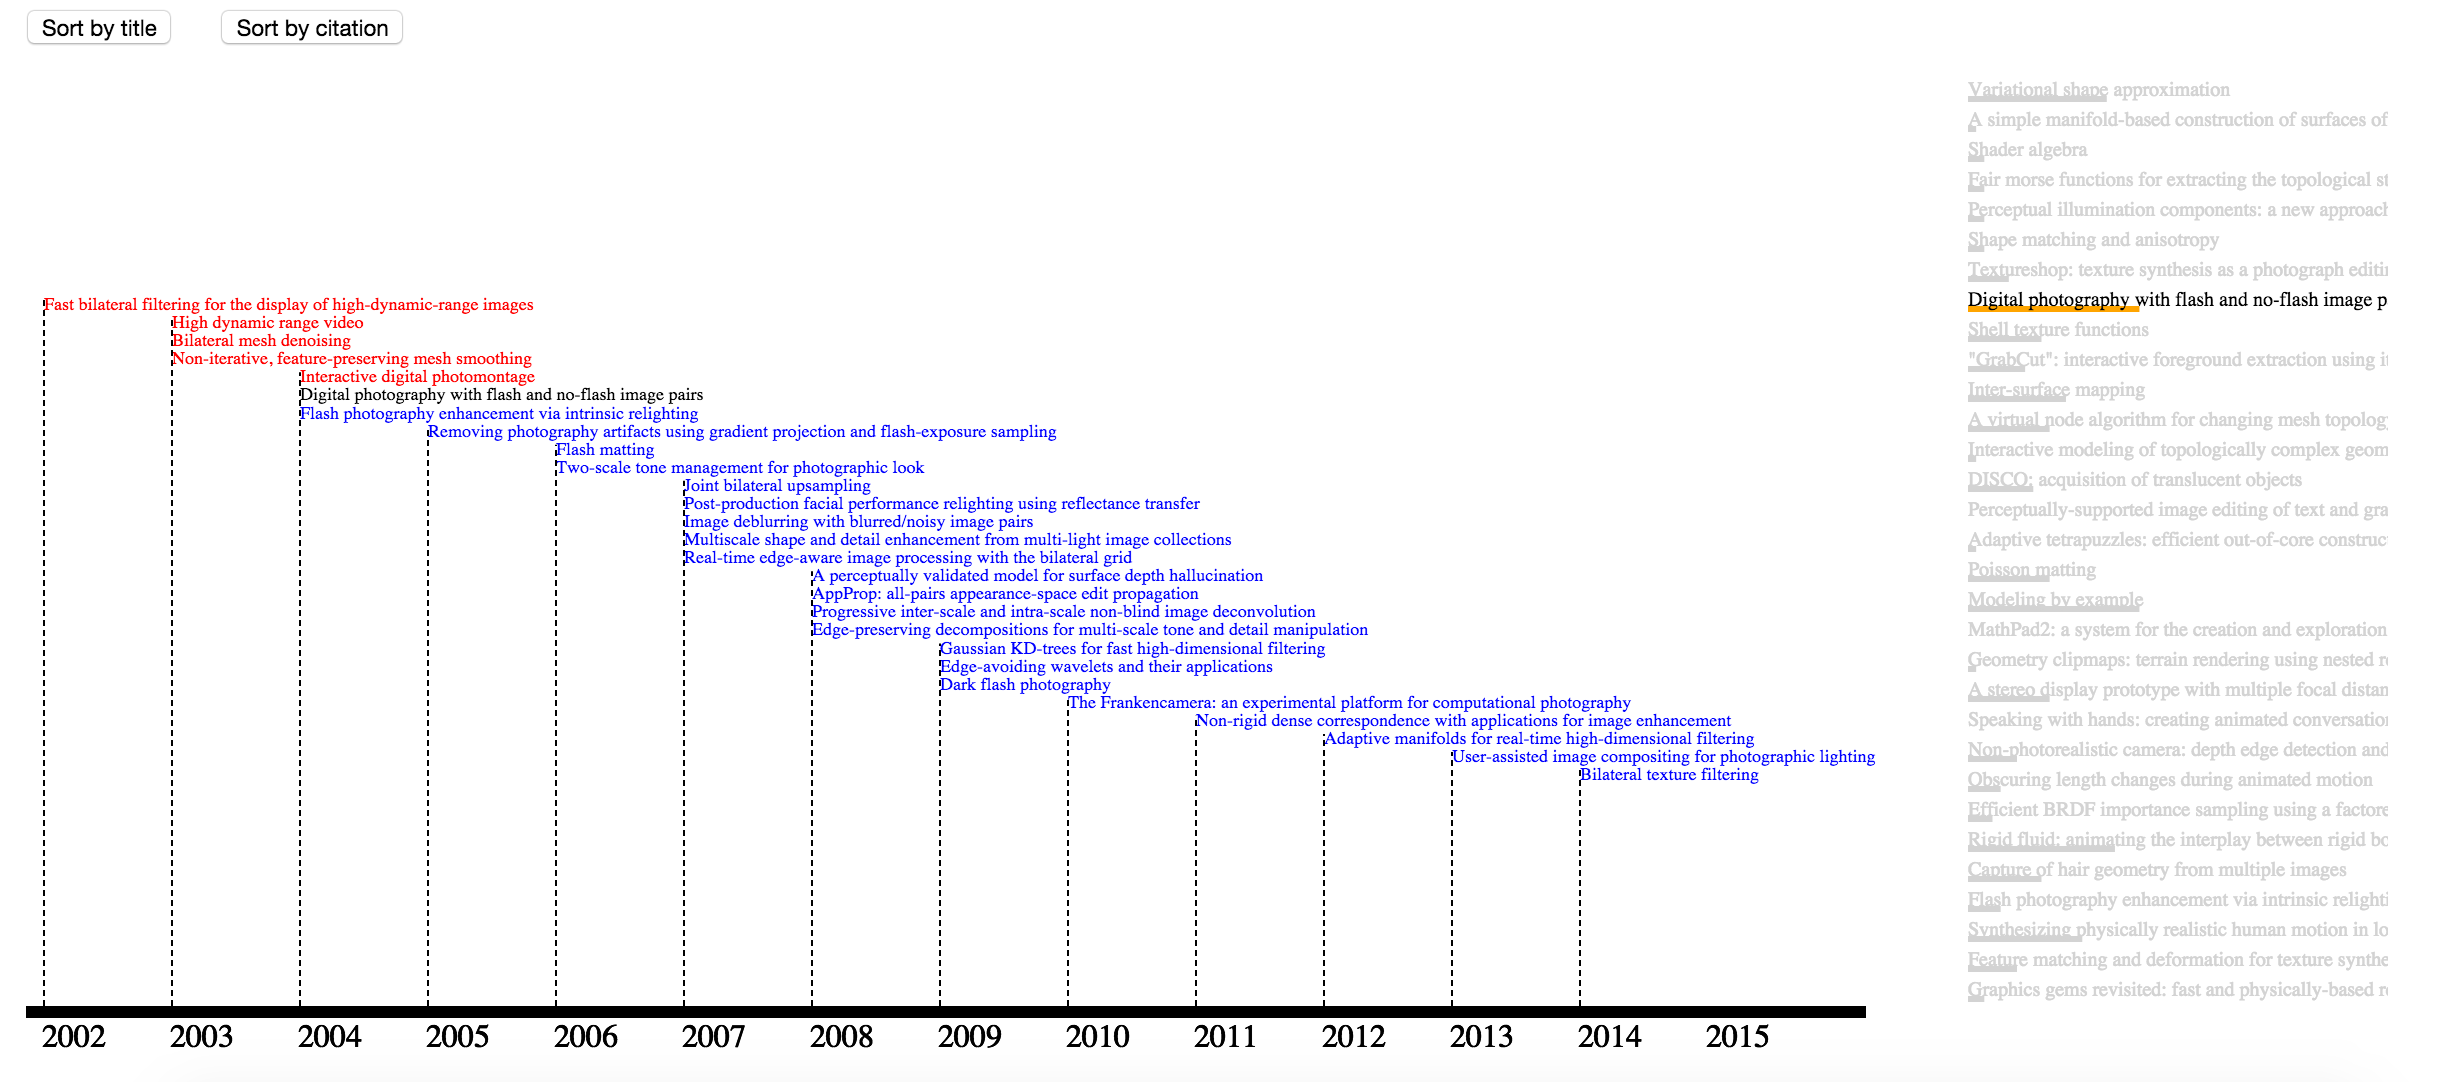
\includegraphics[width=0.7\textwidth]{paper_view_reference_relationship}
	\caption{Paper view with reference and citation for one selected paper}
	\label{fig:pv_reference_citation}
\end{figure} 

Besides that, we also implemented functions, like ``sort title by citation count'' and ``sort title by letter''. More functionalities will be added before final submission.

During implementation, we also realized it is quite difficult to do a university maps view as we promised in the proposal because it is hard to get coordination of universities. So, we decided to get rid of it and add more functionalities to papers view instead, such as searching title. Meanwhile, we can spend more time on keyword view, which we believe is much more useful for users to explore papers. 

